\subsection{Displaysoftware}
\label{subsec:Software_Display}

Das NX8048T070 7-Zoll Display von Nextion wurde mit der dazugehörigen Software \flqq Nextion Editor\frqq~programmiert. Diese wurde eigens für die angebotenen Displaytypen entwickelt und erleichtern dem Benutzer die Erstellung von grafischen Oberflächen und deren Funktion. Die Softwareoberfläche ist in Abbildung \ref{fig:NextionEditor} zu sehen. Der Aufbau ist relativ simpel gestaltet. In der Mitte der Software befindet sich eine grosse Ansicht der bereits Erstellten Displayseite. Darauf sind alle Komponenten zu sehen, welche schon platziert wurden und deren Formatierung. Auf der linken Seite können im oberen Bereich Elemente per Drag and Drop in die Displayseite gezogen werden. Unterhalb der Elementauswahl befindet sich ein Medienfenster, in welchem Bilder für Hintergründe der Elemente, Audiodateien und andere Medien abgespeichert werden können. Auf der rechten Seite im oberen Bereich befindet sich die Seitenansicht, worin alle erstellen Displayseiten sichtbar sind. Die ausgewählte Displayseite erscheint in der Mitte der Software. Um die gewählten Elemente Formatieren zu können, befindet sich im unteren Bereich der rechten Seite ein Fenster mit den möglichen Formatierungen des jeweils gewählten Elementes. Unter der Displayseite gibt es noch ein Output-Fenster und ein Event-Fenster, in welchem die gewünschte Programmierung festgelegt werden kann. Ein cooles Feature des Nextion Editor's ist der Debug-Modus. Mit diesem Tool kann auch ohne Bildschirm die Funktion getestet werden. 

\begin{figure}[h!]
	\centering
	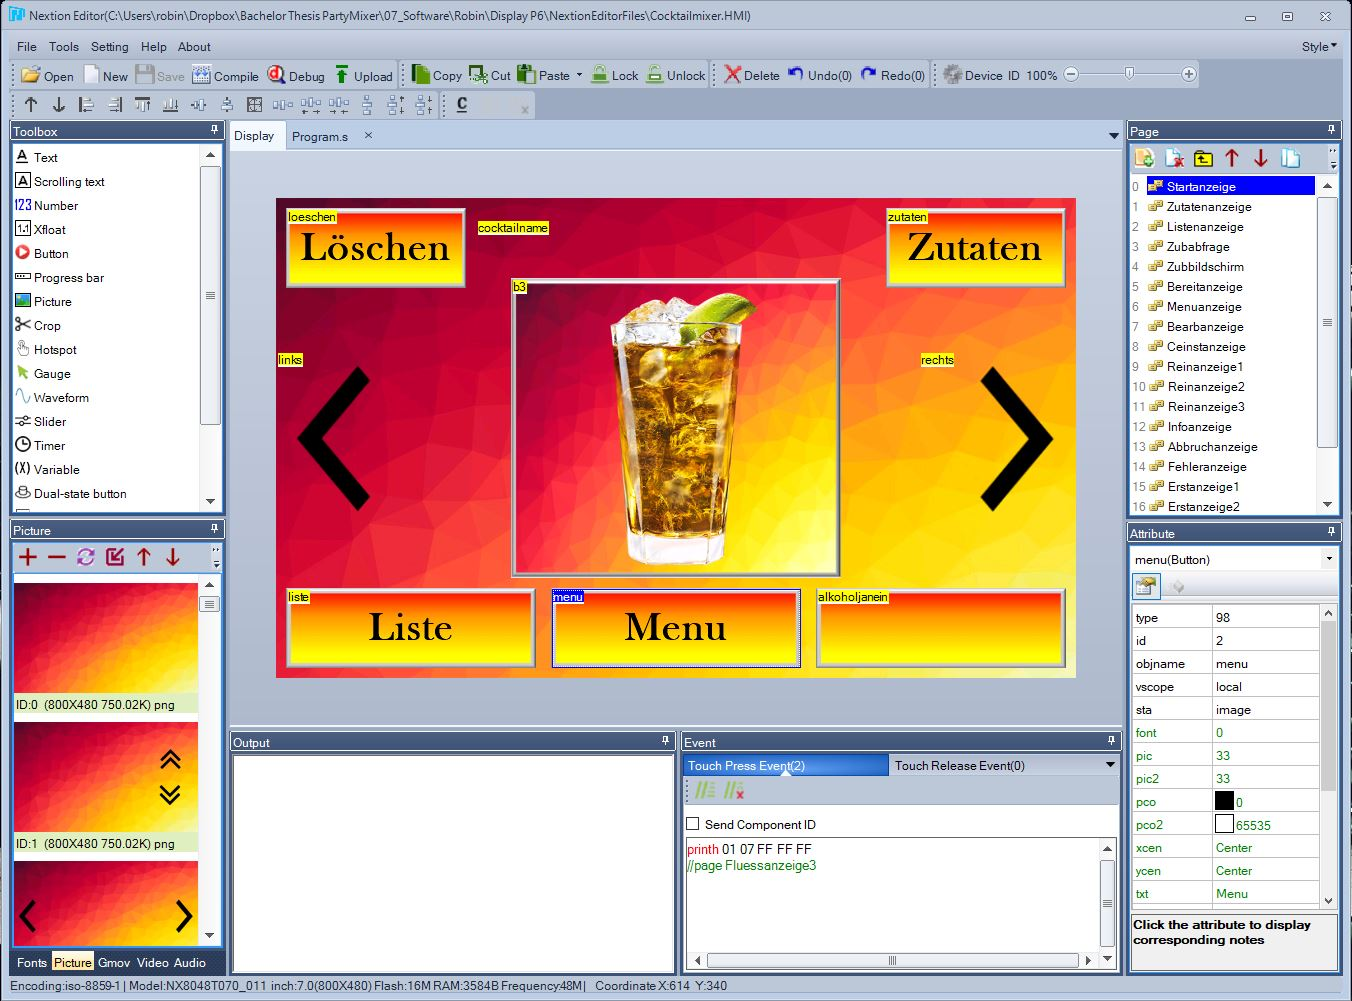
\includegraphics[width=\textwidth]{graphics/NextionEditor}
	\caption{Programmieroberfläche von Nextion}
	\label{fig:NextionEditor}
\end{figure}

\newpage
 


